% Created by tikzDevice version 0.12
% !TEX encoding = UTF-8 Unicode
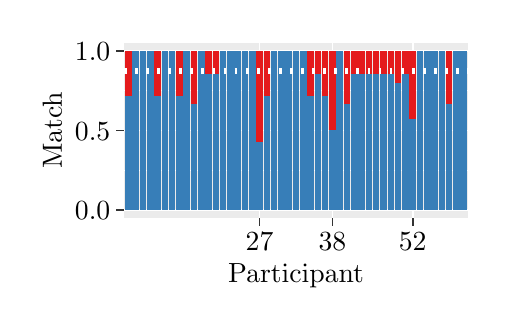
\begin{tikzpicture}[x=1pt,y=1pt]
\definecolor{fillColor}{RGB}{255,255,255}
\path[use as bounding box,fill=fillColor,fill opacity=0.00] (0,0) rectangle (164.64, 99.67);
\begin{scope}
\path[clip] (  0.00,  0.00) rectangle (164.64, 99.67);
\definecolor{drawColor}{RGB}{255,255,255}
\definecolor{fillColor}{RGB}{255,255,255}

\path[draw=drawColor,line width= 0.6pt,line join=round,line cap=round,fill=fillColor] (  0.00,  0.00) rectangle (164.64, 99.67);
\end{scope}
\begin{scope}
\path[clip] ( 34.81, 30.86) rectangle (159.14, 94.17);
\definecolor{fillColor}{gray}{0.92}

\path[fill=fillColor] ( 34.81, 30.86) rectangle (159.14, 94.17);
\definecolor{drawColor}{RGB}{255,255,255}

\path[draw=drawColor,line width= 0.3pt,line join=round] ( 34.81, 48.13) --
	(159.14, 48.13);

\path[draw=drawColor,line width= 0.3pt,line join=round] ( 34.81, 76.91) --
	(159.14, 76.91);

\path[draw=drawColor,line width= 0.6pt,line join=round] ( 34.81, 33.74) --
	(159.14, 33.74);

\path[draw=drawColor,line width= 0.6pt,line join=round] ( 34.81, 62.52) --
	(159.14, 62.52);

\path[draw=drawColor,line width= 0.6pt,line join=round] ( 34.81, 91.29) --
	(159.14, 91.29);

\path[draw=drawColor,line width= 0.6pt,line join=round] ( 83.80, 30.86) --
	( 83.80, 94.17);

\path[draw=drawColor,line width= 0.6pt,line join=round] (110.14, 30.86) --
	(110.14, 94.17);

\path[draw=drawColor,line width= 0.6pt,line join=round] (139.12, 30.86) --
	(139.12, 94.17);
\definecolor{fillColor}{RGB}{55,126,184}

\path[fill=fillColor] ( 35.20, 33.74) rectangle ( 37.57, 74.85);
\definecolor{fillColor}{RGB}{228,26,28}

\path[fill=fillColor] ( 35.20, 74.85) rectangle ( 37.57, 91.29);
\definecolor{fillColor}{RGB}{55,126,184}

\path[fill=fillColor] ( 37.84, 33.74) rectangle ( 40.21, 91.29);

\path[fill=fillColor] ( 40.47, 33.74) rectangle ( 42.84, 91.29);

\path[fill=fillColor] ( 43.10, 33.74) rectangle ( 45.47, 91.29);

\path[fill=fillColor] ( 45.74, 33.74) rectangle ( 48.11, 74.85);
\definecolor{fillColor}{RGB}{228,26,28}

\path[fill=fillColor] ( 45.74, 74.85) rectangle ( 48.11, 91.29);
\definecolor{fillColor}{RGB}{55,126,184}

\path[fill=fillColor] ( 48.37, 33.74) rectangle ( 50.74, 91.29);

\path[fill=fillColor] ( 51.01, 33.74) rectangle ( 53.38, 91.29);

\path[fill=fillColor] ( 53.64, 33.74) rectangle ( 56.01, 74.85);
\definecolor{fillColor}{RGB}{228,26,28}

\path[fill=fillColor] ( 53.64, 74.85) rectangle ( 56.01, 91.29);
\definecolor{fillColor}{RGB}{55,126,184}

\path[fill=fillColor] ( 56.27, 33.74) rectangle ( 58.65, 91.29);

\path[fill=fillColor] ( 58.91, 33.74) rectangle ( 61.28, 72.11);
\definecolor{fillColor}{RGB}{228,26,28}

\path[fill=fillColor] ( 58.91, 72.11) rectangle ( 61.28, 91.29);
\definecolor{fillColor}{RGB}{55,126,184}

\path[fill=fillColor] ( 61.54, 33.74) rectangle ( 63.91, 91.29);

\path[fill=fillColor] ( 64.18, 33.74) rectangle ( 66.55, 83.07);
\definecolor{fillColor}{RGB}{228,26,28}

\path[fill=fillColor] ( 64.18, 83.07) rectangle ( 66.55, 91.29);
\definecolor{fillColor}{RGB}{55,126,184}

\path[fill=fillColor] ( 66.81, 33.74) rectangle ( 69.18, 83.07);
\definecolor{fillColor}{RGB}{228,26,28}

\path[fill=fillColor] ( 66.81, 83.07) rectangle ( 69.18, 91.29);
\definecolor{fillColor}{RGB}{55,126,184}

\path[fill=fillColor] ( 69.45, 33.74) rectangle ( 71.82, 91.29);

\path[fill=fillColor] ( 72.08, 33.74) rectangle ( 74.45, 91.29);

\path[fill=fillColor] ( 74.71, 33.74) rectangle ( 77.08, 91.29);

\path[fill=fillColor] ( 77.35, 33.74) rectangle ( 79.72, 91.29);

\path[fill=fillColor] ( 79.98, 33.74) rectangle ( 82.35, 91.29);

\path[fill=fillColor] ( 82.62, 33.74) rectangle ( 84.99, 58.41);
\definecolor{fillColor}{RGB}{228,26,28}

\path[fill=fillColor] ( 82.62, 58.41) rectangle ( 84.99, 91.29);
\definecolor{fillColor}{RGB}{55,126,184}

\path[fill=fillColor] ( 85.25, 33.74) rectangle ( 87.62, 74.85);
\definecolor{fillColor}{RGB}{228,26,28}

\path[fill=fillColor] ( 85.25, 74.85) rectangle ( 87.62, 91.29);
\definecolor{fillColor}{RGB}{55,126,184}

\path[fill=fillColor] ( 87.88, 33.74) rectangle ( 90.26, 91.29);

\path[fill=fillColor] ( 90.52, 33.74) rectangle ( 92.89, 91.29);

\path[fill=fillColor] ( 93.15, 33.74) rectangle ( 95.52, 91.29);

\path[fill=fillColor] ( 95.79, 33.74) rectangle ( 98.16, 91.29);

\path[fill=fillColor] ( 98.42, 33.74) rectangle (100.79, 91.29);

\path[fill=fillColor] (101.06, 33.74) rectangle (103.43, 74.85);
\definecolor{fillColor}{RGB}{228,26,28}

\path[fill=fillColor] (101.06, 74.85) rectangle (103.43, 91.29);
\definecolor{fillColor}{RGB}{55,126,184}

\path[fill=fillColor] (103.69, 33.74) rectangle (106.06, 83.07);
\definecolor{fillColor}{RGB}{228,26,28}

\path[fill=fillColor] (103.69, 83.07) rectangle (106.06, 91.29);
\definecolor{fillColor}{RGB}{55,126,184}

\path[fill=fillColor] (106.32, 33.74) rectangle (108.70, 74.85);
\definecolor{fillColor}{RGB}{228,26,28}

\path[fill=fillColor] (106.32, 74.85) rectangle (108.70, 91.29);
\definecolor{fillColor}{RGB}{55,126,184}

\path[fill=fillColor] (108.96, 33.74) rectangle (111.33, 62.52);
\definecolor{fillColor}{RGB}{228,26,28}

\path[fill=fillColor] (108.96, 62.52) rectangle (111.33, 91.29);
\definecolor{fillColor}{RGB}{55,126,184}

\path[fill=fillColor] (111.59, 33.74) rectangle (113.96, 91.29);

\path[fill=fillColor] (114.23, 33.74) rectangle (116.60, 72.11);
\definecolor{fillColor}{RGB}{228,26,28}

\path[fill=fillColor] (114.23, 72.11) rectangle (116.60, 91.29);
\definecolor{fillColor}{RGB}{55,126,184}

\path[fill=fillColor] (116.86, 33.74) rectangle (119.23, 83.07);
\definecolor{fillColor}{RGB}{228,26,28}

\path[fill=fillColor] (116.86, 83.07) rectangle (119.23, 91.29);
\definecolor{fillColor}{RGB}{55,126,184}

\path[fill=fillColor] (119.50, 33.74) rectangle (121.87, 83.07);
\definecolor{fillColor}{RGB}{228,26,28}

\path[fill=fillColor] (119.50, 83.07) rectangle (121.87, 91.29);
\definecolor{fillColor}{RGB}{55,126,184}

\path[fill=fillColor] (122.13, 33.74) rectangle (124.50, 83.07);
\definecolor{fillColor}{RGB}{228,26,28}

\path[fill=fillColor] (122.13, 83.07) rectangle (124.50, 91.29);
\definecolor{fillColor}{RGB}{55,126,184}

\path[fill=fillColor] (124.76, 33.74) rectangle (127.13, 83.07);
\definecolor{fillColor}{RGB}{228,26,28}

\path[fill=fillColor] (124.76, 83.07) rectangle (127.13, 91.29);
\definecolor{fillColor}{RGB}{55,126,184}

\path[fill=fillColor] (127.40, 33.74) rectangle (129.77, 83.07);
\definecolor{fillColor}{RGB}{228,26,28}

\path[fill=fillColor] (127.40, 83.07) rectangle (129.77, 91.29);
\definecolor{fillColor}{RGB}{55,126,184}

\path[fill=fillColor] (130.03, 33.74) rectangle (132.40, 83.07);
\definecolor{fillColor}{RGB}{228,26,28}

\path[fill=fillColor] (130.03, 83.07) rectangle (132.40, 91.29);
\definecolor{fillColor}{RGB}{55,126,184}

\path[fill=fillColor] (132.67, 33.74) rectangle (135.04, 79.78);
\definecolor{fillColor}{RGB}{228,26,28}

\path[fill=fillColor] (132.67, 79.78) rectangle (135.04, 91.29);
\definecolor{fillColor}{RGB}{55,126,184}

\path[fill=fillColor] (135.30, 33.74) rectangle (137.67, 83.07);
\definecolor{fillColor}{RGB}{228,26,28}

\path[fill=fillColor] (135.30, 83.07) rectangle (137.67, 91.29);
\definecolor{fillColor}{RGB}{55,126,184}

\path[fill=fillColor] (137.93, 33.74) rectangle (140.31, 66.63);
\definecolor{fillColor}{RGB}{228,26,28}

\path[fill=fillColor] (137.93, 66.63) rectangle (140.31, 91.29);
\definecolor{fillColor}{RGB}{55,126,184}

\path[fill=fillColor] (140.57, 33.74) rectangle (142.94, 91.29);

\path[fill=fillColor] (143.20, 33.74) rectangle (145.57, 91.29);

\path[fill=fillColor] (145.84, 33.74) rectangle (148.21, 91.29);

\path[fill=fillColor] (148.47, 33.74) rectangle (150.84, 91.29);

\path[fill=fillColor] (151.11, 33.74) rectangle (153.48, 72.11);
\definecolor{fillColor}{RGB}{228,26,28}

\path[fill=fillColor] (151.11, 72.11) rectangle (153.48, 91.29);
\definecolor{fillColor}{RGB}{55,126,184}

\path[fill=fillColor] (153.74, 33.74) rectangle (156.11, 91.29);

\path[fill=fillColor] (156.37, 33.74) rectangle (158.74, 91.29);

\path[draw=drawColor,line width= 2.3pt,dash pattern=on 1pt off 3pt ,line join=round] ( 34.81, 83.98) -- (159.14, 83.98);
\end{scope}
\begin{scope}
\path[clip] (  0.00,  0.00) rectangle (164.64, 99.67);
\definecolor{drawColor}{RGB}{0,0,0}

\node[text=drawColor,anchor=base east,inner sep=0pt, outer sep=0pt, scale=  1.00] at ( 29.86, 30.30) {0.0};

\node[text=drawColor,anchor=base east,inner sep=0pt, outer sep=0pt, scale=  1.00] at ( 29.86, 59.07) {0.5};

\node[text=drawColor,anchor=base east,inner sep=0pt, outer sep=0pt, scale=  1.00] at ( 29.86, 87.85) {1.0};
\end{scope}
\begin{scope}
\path[clip] (  0.00,  0.00) rectangle (164.64, 99.67);
\definecolor{drawColor}{gray}{0.20}

\path[draw=drawColor,line width= 0.6pt,line join=round] ( 32.06, 33.74) --
	( 34.81, 33.74);

\path[draw=drawColor,line width= 0.6pt,line join=round] ( 32.06, 62.52) --
	( 34.81, 62.52);

\path[draw=drawColor,line width= 0.6pt,line join=round] ( 32.06, 91.29) --
	( 34.81, 91.29);
\end{scope}
\begin{scope}
\path[clip] (  0.00,  0.00) rectangle (164.64, 99.67);
\definecolor{drawColor}{gray}{0.20}

\path[draw=drawColor,line width= 0.6pt,line join=round] ( 83.80, 28.11) --
	( 83.80, 30.86);

\path[draw=drawColor,line width= 0.6pt,line join=round] (110.14, 28.11) --
	(110.14, 30.86);

\path[draw=drawColor,line width= 0.6pt,line join=round] (139.12, 28.11) --
	(139.12, 30.86);
\end{scope}
\begin{scope}
\path[clip] (  0.00,  0.00) rectangle (164.64, 99.67);
\definecolor{drawColor}{RGB}{0,0,0}

\node[text=drawColor,anchor=base,inner sep=0pt, outer sep=0pt, scale=  1.00] at ( 83.80, 19.03) {27};

\node[text=drawColor,anchor=base,inner sep=0pt, outer sep=0pt, scale=  1.00] at (110.14, 19.03) {38};

\node[text=drawColor,anchor=base,inner sep=0pt, outer sep=0pt, scale=  1.00] at (139.12, 19.03) {52};
\end{scope}
\begin{scope}
\path[clip] (  0.00,  0.00) rectangle (164.64, 99.67);
\definecolor{drawColor}{RGB}{0,0,0}

\node[text=drawColor,anchor=base,inner sep=0pt, outer sep=0pt, scale=  1.00] at ( 96.97,  7.44) {Participant};
\end{scope}
\begin{scope}
\path[clip] (  0.00,  0.00) rectangle (164.64, 99.67);
\definecolor{drawColor}{RGB}{0,0,0}

\node[text=drawColor,rotate= 90.00,anchor=base,inner sep=0pt, outer sep=0pt, scale=  1.00] at ( 12.39, 62.52) {Match};
\end{scope}
\end{tikzpicture}
